\subsection{Esecuzione test}

\begin{figure}[H]
    \centering
    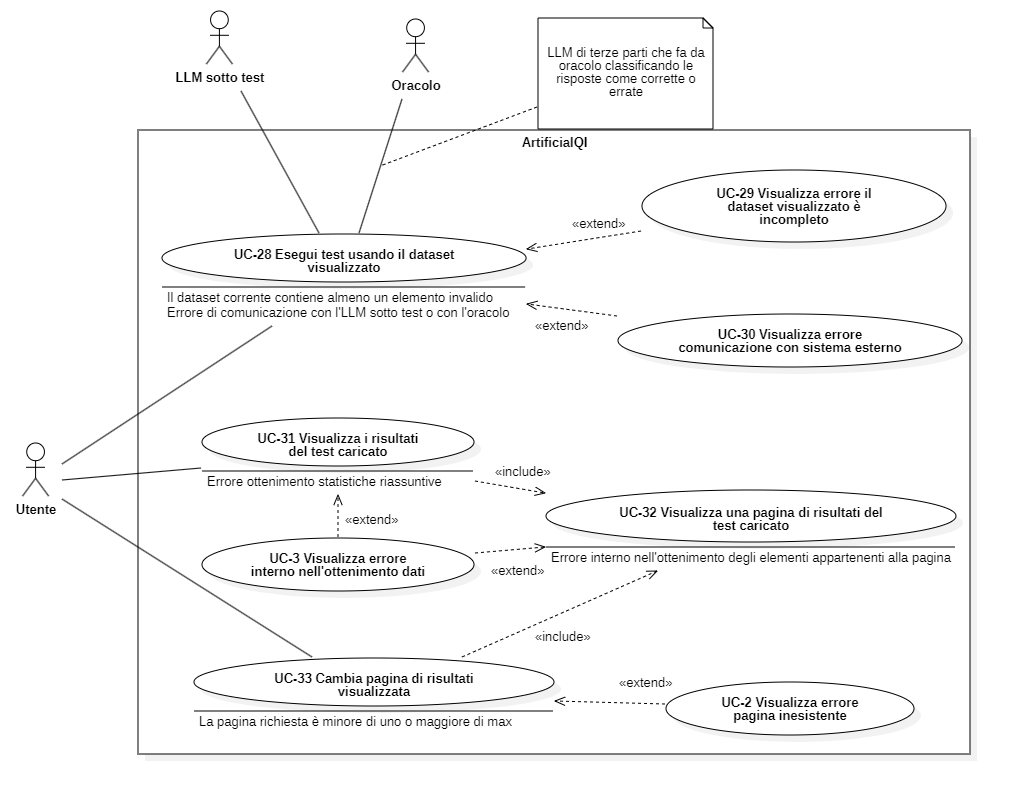
\includegraphics[scale=0.2]{Sezioni/UseCase/Immagini/EsecuzioneTest.png}
    \caption{Diagramma esecuzione test.}
\end{figure}

\begin{usecase}{UC-31}{Esegui test usando il dataset visualizzato}
    \label{uc:UC-31}
    
    \req{\hyperref[ru:RUO-7]{RUO-7}} 

    \pre{
        \item L'utente sta visualizzando il dataset da utilizzare per il test \hyperref[uc:UC-1]{UC-1}
        \item Il dataset visualizzato non è vuoto
    }

    \post{
        \item L'utente visualizza i risultati del test
    }
    
    \actor{Utente}

    \subactors{LLM sotto test, Oracolo}

    \trigger{L'utente vuole eseguire il test usando il dataset visualizzato}

    \inc{}

    \base{}

    \scenario{
        \item L'utente richiede di eseguire il test 
        \item L'utente seleziona un LLM da testare tra quelli salvati nel sistema
        \item Il sistema ottiene le risposte date dal LLM sotto test alle domande contenute nel dataset 
        \item Il sistema chiede all'oracolo la correttezza delle risposte
        \item Il sistema elabora i risultati del test
        \item I risultati del test vengono caricati come correnti
    }

    \subscenario{
        \item[1.1] Il dataset visualizzato contiene almeno un elemento incompleto ovvero con domanda o risposta vuote:
        \begin{itemize}
            \item \hyperref[uc:UC-32]{UC-32}
        \end{itemize}
        \item[2.1] Il sistema riscontra un errore di comunicazione con l'LLM sotto test:
        \begin{itemize}
            \item \hyperref[uc:UC-33]{UC-33}
        \end{itemize}
        \item[3.1] Il sistema riscontra un errore di comunicazione con l'oracolo:
        \begin{itemize}
            \item \hyperref[uc:UC-33]{UC-33}
        \end{itemize}
    }
\end{usecase}

\begin{usecase}{UC-32}{Visualizza errore dataset visualizzato è incompelto}
    \label{uc:UC-32}
    
    \req{} 

    \pre{
        \item Il dataset visualizzato contiene uno o più elementi con domanda o risposta vuote
    }

    \post{
        \item L'utente ottiene dei link alle pagine del dataset che contengono gli elementi incompleti
    }
    
    \actor{Utente}

    \trigger{Il sistema prima di eseguire il test individua elementi incompleti nel dataset}

    \inc{}

    \base{}

    \scenario{
        \item Viene visualizzata una lista di link alle pagine del dataset che contengono gli elementi incompleti evidenziati
    }

    \subscenario{}
\end{usecase}

\begin{usecase}{UC-33}{Visualizza errore di comunicazione con sistema esterno}
    \label{uc:UC-33}
    
    \req{} 

    \pre{
        \item Il sistema interroga un sistema esterno e la comunicazione termina in modo anomalo
    }

    \post{
        \item L'utente viene messo al corrente dell'errore di comunicazione
    }
    
    \actor{Attore}

    \trigger{Il sistema riscontra un errore di comunicazione con un sistema esterno}

    \inc{}

    \base{}

    \scenario{
        \item Viene visualizzato un errore che specifica l'errore di comunicazione
    }

    \subscenario{}
\end{usecase}

\begin{usecase}{UC-34}{Visualizza i risultati del test caricato}
    \label{uc:UC-34}
    
    \req{\hyperref[ru:RUO-8]{RUO-8}} 

    \pre{
        \item Il test di cui si vuole visualizzare i risultati è stato caricato
    }

    \post{
        \item Vengono visualizzati i risultati del test caricato
    }
    
    \actor{Utente}

    \trigger{L'utente vuole visualizzare i risultati del test caricato}

    \inc{\hyperref[uc:UC-35]{UC-35}}

    \base{}

    \scenario{
        \item L'utente richiede la visualizzazione dei risultati del test caricato
        \item Viene visualizzata una dashboard contenente le statistiche sui risultati del test
        \item Viene visualizzata la prima pagina dei risultati del test seguendo \hyperref[uc:UC-35]{UC-35}
    }

    \subscenario{
        \item[2.1] Il sistema riscontra un errore durante l'ottenimento delle statistiche sui risultati del test:
        \begin{itemize}
            \item \hyperref[uc:UC-3]{UC-3}
        \end{itemize}
    }
\end{usecase}


\begin{usecase}{UC-35}{Visualizza pagina di risultati del test caricato}
    \label{uc:UC-35}
    
    \req{} 

    \pre{}

    \post{
        \item Viene visualizzata la pagina dei risultati del test caricato richiesta
    }
    
    \actor{Utente}

    \subactors{}

    \trigger{Il sistema deve visualizzare una precisa pagina dei risultati del test caricato}

    \inc{}

    \base{}

    \scenario{
        \item Il sistema ottiene i risultati del test per la pagina richiesta
        \item Il sistema mostra un diagramma di dispersione che rappresenta i singoli risultati della pagina sotto forma di punti 
        \item Viene visualizzata la lista dei singoli risultati appartenenti alla pagina richiesta
    }

    \subscenario{
        \item[1.1] Il sistema riscontra un errore interno durante l'ottenimento dei risultati appartenenti alla pagina da visualizzare:
        \begin{itemize}
            \item \hyperref[uc:UC-3]{UC-3}
        \end{itemize}
    }
\end{usecase}


\begin{usecase}{UC-36}{Cambia pagina di risultati visualizzata}
    \label{uc:UC-36}
    
    \req{} 

    \pre{
        \item L'utente sta visualizzando i risultati del test caricato
    }

    \post{
        \item Viene visualizzata la pagina dei risultati del test caricato richiesta
    }
    
    \actor{Utente}

    \subactors{}

    \trigger{L'utente vuole visualizzare una pagina dei risultati del test caricato}

    \inc{\hyperref[uc:UC-35]{UC-35}}

    \base{}

    \scenario{
        \item L'utente richiede la visualizzazione di una pagina di risultati del test
        \item Il sistema verifica che la pagina esista
        \item Il sistema visualizza la pagina richiesta seguendo \hyperref[uc:UC-35]{UC-35}
    }

    \subscenario{
        \item[2.1] La pagina richiesta è invalida ovvero minore di uno o maggiore della pagina massima:
        \begin{itemize}
            \item \hyperref[uc:UC-5]{UC-5}
        \end{itemize}
    }
\end{usecase}